% ==========================================================================
% INFO 4617 Web Data Science -- Week 7: Archived Web Pages & the Wayback
% Machine (Chapter 7)
% Build:  latexmk -pdf week-07.tex   (from this folder; no env vars needed)
% (or run `make` from the slides/ directory to build every deck)
% ==========================================================================
\documentclass[9pt,aspectratio=169]{beamer}
% Resolve the shared theme/preamble in ../common/ when compiling this
% file directly from its own folder (no TEXINPUTS needed).
\makeatletter\def\input@path{{../common/}}\makeatother
% ==========================================================================
% Shared preamble for INFO 4617 Web Data Science weekly lecture decks
% Based on the Gotham beamer theme (vendored in this directory).
% Each week's slides.tex does:  % ==========================================================================
% Shared preamble for INFO 4617 Web Data Science weekly lecture decks
% Based on the Gotham beamer theme (vendored in this directory).
% Each week's slides.tex does:  % ==========================================================================
% Shared preamble for INFO 4617 Web Data Science weekly lecture decks
% Based on the Gotham beamer theme (vendored in this directory).
% Each week's slides.tex does:  \input{preamble}  (with common/ on TEXINPUTS)
% then sets \title/\subtitle/\author/\date and \begin{document}.
% ==========================================================================

\usetheme{gotham}

\usepackage{fbb}
\usepackage{booktabs}
\usepackage{graphicx}
\usepackage{tikz}
\usepackage{xcolor}
\usepackage{multirow}
\usepackage{listings}
\usetikzlibrary{positioning, arrows.meta, shapes}

% Bibliography
\usepackage[style=authoryear,
            backend=biber,
            maxcitenames=1,
            uniquename=false,
            uniquelist=false]{biblatex}
\addbibresource{bibliography.bib}

\gothamset{sectiontocframe default=off}

% ------------------------------------------------------------------ colors
\definecolor{cugold}{HTML}{CFB87C}
\definecolor{tab-red}{HTML}{E15759}
\definecolor{tab-orange}{HTML}{F28E2B}
\definecolor{tab-blue}{HTML}{4E79A7}
\definecolor{tab-cyan}{HTML}{76B7B2}
\definecolor{tab-green}{HTML}{59A14F}
\definecolor{tab-yellow}{HTML}{EDC948}
\definecolor{tab-purple}{HTML}{B07AA1}
\definecolor{tab-pink}{HTML}{FF9DA7}
\definecolor{tab-brown}{HTML}{9C755F}
\definecolor{tab-gray}{HTML}{BAB0AC}

\setbeamercolor{frametitle}{fg=black, bg=cugold}
\setbeamercolor{progress bar}{fg=cugold, bg=cugold!20}

\setbeamercolor{block title alerted}{fg=black, bg=cugold}
\setbeamercolor{block body alerted}{fg=black, bg=cugold!10}

% ------------------------------------------------------------------ footline
\setbeamertemplate{footline}{
  \begin{beamercolorbox}[wd=\paperwidth,ht=2.5ex,dp=1ex,right]{footline}
    {\footnotesize \insertframenumber{} of \inserttotalframenumber}
    \hspace*{2ex}
  \end{beamercolorbox}
}

% ------------------------------------------------------------------ helpers
\newcommand{\bottomcite}[1]{
    \vspace*{\fill}
    \vspace{-\baselineskip}
    {\tiny
    \rule{\textwidth}{0.3pt}\\
    #1
    }
    \vspace{0.5ex}
}

% Consistent code styling for the Wednesday "applied notebook" frames.
\lstdefinestyle{wds}{
    basicstyle=\ttfamily\scriptsize,
    keywordstyle=\color{tab-blue}\bfseries,
    commentstyle=\color{tab-green},
    stringstyle=\color{tab-orange},
    showstringspaces=false,
    breaklines=true,
    columns=fullflexible,
    language=Python,
    aboveskip=0.4em,
    belowskip=0.4em,
}
\lstset{style=wds}

% \dayband{Day}{Topic} -- a lightweight section divider label used to mark
% Monday / Wednesday / Friday within a week's deck.
\newcommand{\dayband}[2]{{\large\textbf{#1}}\;\textcolor{tab-gray}{\textbar}\;#2}
  (with common/ on TEXINPUTS)
% then sets \title/\subtitle/\author/\date and \begin{document}.
% ==========================================================================

\usetheme{gotham}

\usepackage{fbb}
\usepackage{booktabs}
\usepackage{graphicx}
\usepackage{tikz}
\usepackage{xcolor}
\usepackage{multirow}
\usepackage{listings}
\usetikzlibrary{positioning, arrows.meta, shapes}

% Bibliography
\usepackage[style=authoryear,
            backend=biber,
            maxcitenames=1,
            uniquename=false,
            uniquelist=false]{biblatex}
\addbibresource{bibliography.bib}

\gothamset{sectiontocframe default=off}

% ------------------------------------------------------------------ colors
\definecolor{cugold}{HTML}{CFB87C}
\definecolor{tab-red}{HTML}{E15759}
\definecolor{tab-orange}{HTML}{F28E2B}
\definecolor{tab-blue}{HTML}{4E79A7}
\definecolor{tab-cyan}{HTML}{76B7B2}
\definecolor{tab-green}{HTML}{59A14F}
\definecolor{tab-yellow}{HTML}{EDC948}
\definecolor{tab-purple}{HTML}{B07AA1}
\definecolor{tab-pink}{HTML}{FF9DA7}
\definecolor{tab-brown}{HTML}{9C755F}
\definecolor{tab-gray}{HTML}{BAB0AC}

\setbeamercolor{frametitle}{fg=black, bg=cugold}
\setbeamercolor{progress bar}{fg=cugold, bg=cugold!20}

\setbeamercolor{block title alerted}{fg=black, bg=cugold}
\setbeamercolor{block body alerted}{fg=black, bg=cugold!10}

% ------------------------------------------------------------------ footline
\setbeamertemplate{footline}{
  \begin{beamercolorbox}[wd=\paperwidth,ht=2.5ex,dp=1ex,right]{footline}
    {\footnotesize \insertframenumber{} of \inserttotalframenumber}
    \hspace*{2ex}
  \end{beamercolorbox}
}

% ------------------------------------------------------------------ helpers
\newcommand{\bottomcite}[1]{
    \vspace*{\fill}
    \vspace{-\baselineskip}
    {\tiny
    \rule{\textwidth}{0.3pt}\\
    #1
    }
    \vspace{0.5ex}
}

% Consistent code styling for the Wednesday "applied notebook" frames.
\lstdefinestyle{wds}{
    basicstyle=\ttfamily\scriptsize,
    keywordstyle=\color{tab-blue}\bfseries,
    commentstyle=\color{tab-green},
    stringstyle=\color{tab-orange},
    showstringspaces=false,
    breaklines=true,
    columns=fullflexible,
    language=Python,
    aboveskip=0.4em,
    belowskip=0.4em,
}
\lstset{style=wds}

% \dayband{Day}{Topic} -- a lightweight section divider label used to mark
% Monday / Wednesday / Friday within a week's deck.
\newcommand{\dayband}[2]{{\large\textbf{#1}}\;\textcolor{tab-gray}{\textbar}\;#2}
  (with common/ on TEXINPUTS)
% then sets \title/\subtitle/\author/\date and \begin{document}.
% ==========================================================================

\usetheme{gotham}

\usepackage{fbb}
\usepackage{booktabs}
\usepackage{graphicx}
\usepackage{tikz}
\usepackage{xcolor}
\usepackage{multirow}
\usepackage{listings}
\usetikzlibrary{positioning, arrows.meta, shapes}

% Bibliography
\usepackage[style=authoryear,
            backend=biber,
            maxcitenames=1,
            uniquename=false,
            uniquelist=false]{biblatex}
\addbibresource{bibliography.bib}

\gothamset{sectiontocframe default=off}

% ------------------------------------------------------------------ colors
\definecolor{cugold}{HTML}{CFB87C}
\definecolor{tab-red}{HTML}{E15759}
\definecolor{tab-orange}{HTML}{F28E2B}
\definecolor{tab-blue}{HTML}{4E79A7}
\definecolor{tab-cyan}{HTML}{76B7B2}
\definecolor{tab-green}{HTML}{59A14F}
\definecolor{tab-yellow}{HTML}{EDC948}
\definecolor{tab-purple}{HTML}{B07AA1}
\definecolor{tab-pink}{HTML}{FF9DA7}
\definecolor{tab-brown}{HTML}{9C755F}
\definecolor{tab-gray}{HTML}{BAB0AC}

\setbeamercolor{frametitle}{fg=black, bg=cugold}
\setbeamercolor{progress bar}{fg=cugold, bg=cugold!20}

\setbeamercolor{block title alerted}{fg=black, bg=cugold}
\setbeamercolor{block body alerted}{fg=black, bg=cugold!10}

% ------------------------------------------------------------------ footline
\setbeamertemplate{footline}{
  \begin{beamercolorbox}[wd=\paperwidth,ht=2.5ex,dp=1ex,right]{footline}
    {\footnotesize \insertframenumber{} of \inserttotalframenumber}
    \hspace*{2ex}
  \end{beamercolorbox}
}

% ------------------------------------------------------------------ helpers
\newcommand{\bottomcite}[1]{
    \vspace*{\fill}
    \vspace{-\baselineskip}
    {\tiny
    \rule{\textwidth}{0.3pt}\\
    #1
    }
    \vspace{0.5ex}
}

% Consistent code styling for the Wednesday "applied notebook" frames.
\lstdefinestyle{wds}{
    basicstyle=\ttfamily\scriptsize,
    keywordstyle=\color{tab-blue}\bfseries,
    commentstyle=\color{tab-green},
    stringstyle=\color{tab-orange},
    showstringspaces=false,
    breaklines=true,
    columns=fullflexible,
    language=Python,
    aboveskip=0.4em,
    belowskip=0.4em,
}
\lstset{style=wds}

% \dayband{Day}{Topic} -- a lightweight section divider label used to mark
% Monday / Wednesday / Friday within a week's deck.
\newcommand{\dayband}[2]{{\large\textbf{#1}}\;\textcolor{tab-gray}{\textbar}\;#2}


\title[Week 7 · Web Archives]{{\Huge Archived Web Pages \& the Wayback Machine}}
\subtitle{Week 7 · Documents module · Textbook Chapter 7}
\author[Keegan]{\textbf{Brian C. Keegan, Ph.D.} \\ Associate Professor, Department of Information Science \\ University of Colorado Boulder}
\date{September 28, 30 \& October 2, 2026}

\begin{document}

\maketitle

% -------------------------------------------------------------------------
\begin{frame}{This week at a glance}
    \begin{columns}
        \begin{column}{0.6\textwidth}
            The web is not permanent. This week we scrape the \textit{past} --- and measure how pages change over time.

            \bigskip

            \dayband{Monday}{Concepts \& notebook intro}
            \begin{itemize}\small
                \item Web archiving, the Wayback Machine by hand, how captures break, and what researchers do with them
            \end{itemize}

            \medskip

            \dayband{Wednesday}{Notebook lab}
            \begin{itemize}\small
                \item Work the Chapter 7 notebook: Availability API, CDX, tracking a Terms-of-Service document
            \end{itemize}

            \medskip

            \dayband{Friday}{Textbook revisions}
            \begin{itemize}\small
                \item Propose \& peer-review pull requests improving Chapter 7
            \end{itemize}
        \end{column}
        \begin{column}{0.35\textwidth}
            \begin{block}{Companion notebook}
                \footnotesize \texttt{ch-07-archives.ipynb}
            \end{block}
            \begin{alertblock}{Bring a laptop}
                \footnotesize Monday and Wednesday are both hands-on this week --- bring a laptop both days.
            \end{alertblock}
        \end{column}
    \end{columns}
\end{frame}

% =========================================================================
\section{Monday · Concepts}
% =========================================================================

\begin{frame}{Link rot}
    \begin{columns}
        \begin{column}{0.6\textwidth}
            38\% of the web pages that existed in 2013 were gone a decade later.

            \bigskip
            Usually the website is still up --- one page on it was deleted or removed.

            \bigskip
            How do you study something that might not be there tomorrow?

            \bigskip
            How do you measure a \textit{change} when you can only see today's version?
        \end{column}
        \begin{column}{0.35\textwidth}
            \centering
            
\includegraphics[width=\textwidth]{slides/week-07/img/i-dont-feel-so-good.jpg}\\
            {\footnotesize Web pages after a decade or so}
        \end{column}
    \end{columns}
\end{frame}

\begin{frame}{Web archiving}
    \begin{center}
        
\includegraphics[width=.7\textwidth]{img/wayback_trillion.png}
    \end{center}

    \textbf{Web archiving}: collect pages as they looked at a moment, store them, and let anyone replay them later.

    \bigskip
    The \textbf{Internet Archive} is a nonprofit library Brewster Kahle founded in 1996. Its \textbf{Wayback Machine} opened to the public in 2001. In October 2025 it passed \textbf{one trillion} archived web pages.

    \bigskip
    National libraries and universities archive the web too. The Wayback Machine is the one anyone can search: \url{https://web.archive.org}
\end{frame}

\begin{frame}{Finding a capture}
    \begin{center}
        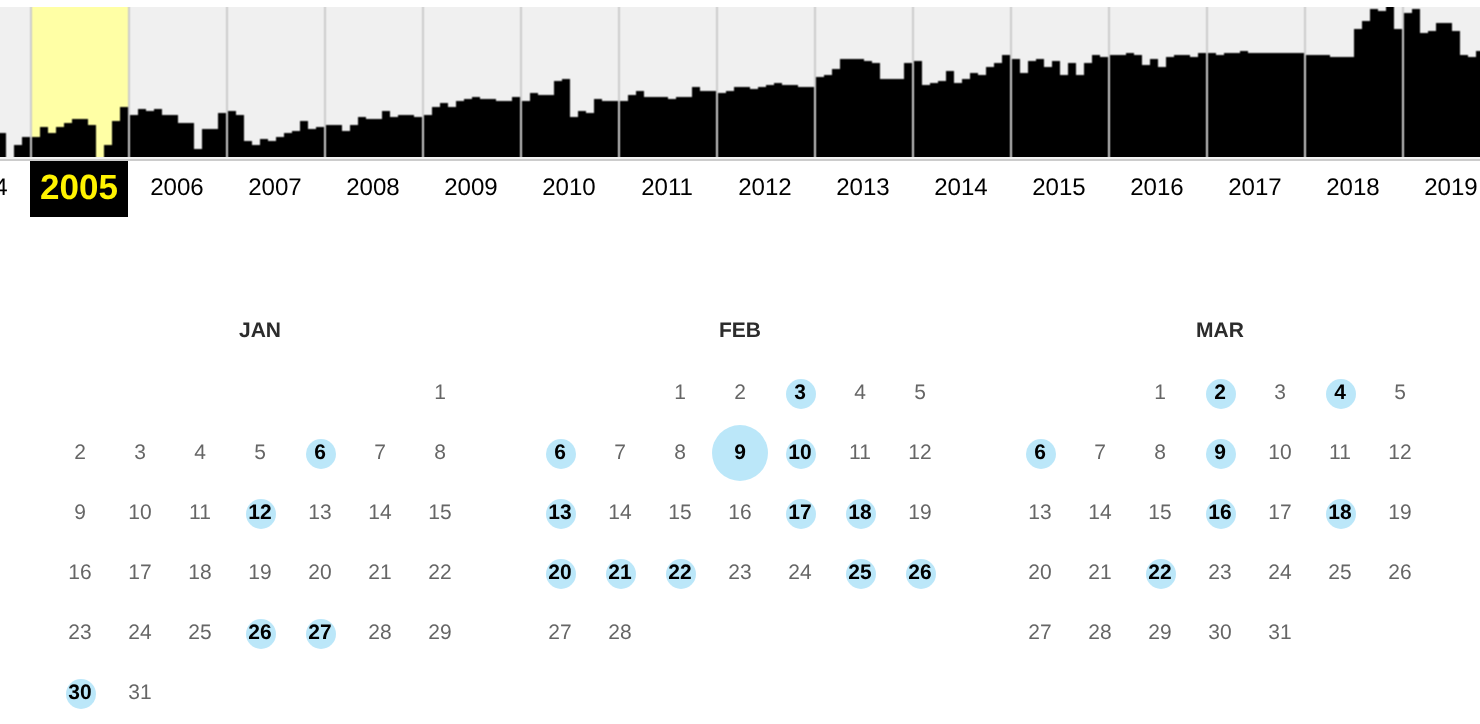
\includegraphics[width=.72\textwidth]{img/wayback_calendar.png}
    \end{center}

    Type a URL into \url{https://web.archive.org}. The bars across the top are the years --- taller means more captures that year.

    \bigskip
    Click a year for its calendar. Each dot is a day with captures, and a bigger dot means more of them. Hover a dot to list that day's capture times.
\end{frame}

\begin{frame}{Moving through time}
    \begin{center}
        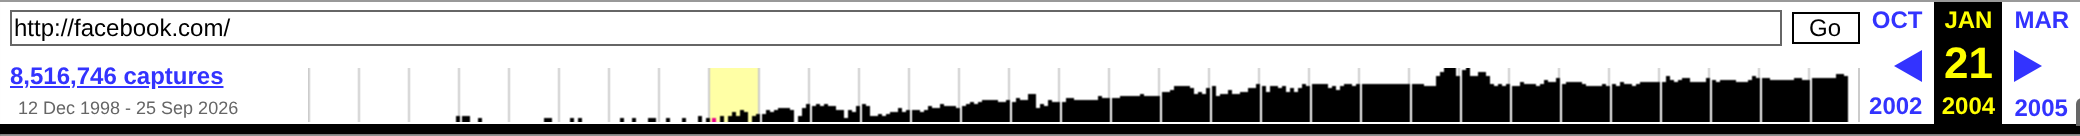
\includegraphics[width=\textwidth]{img/toolbar.png}
    \end{center}

    Every capture opens with this toolbar: the URL, how many times it was captured, and a strip of bars across the years.

    \bigskip
    Click anywhere on the strip to jump to that moment. The arrows and the neighboring months and years step you backward and forward.

    \bigskip
    The big yellow date is the capture on screen --- here, facebook.com on January 21, 2004.
\end{frame}

\begin{frame}{The URL is the query}
    \begin{center}
        
\includegraphics[width=.8\textwidth]{img/address_bar.png}
    \end{center}

    The 14 digits are a timestamp in UTC: year, month, day, hour, minute, second. \texttt{20040212031928} is February 12, 2004, at 03:19:28.

    \bigskip
    Shorten it and the Archive finds the closest capture: \texttt{web.archive.org/web/2004/thefacebook.com}

    \bigskip
    Add a star for a calendar, \texttt{/web/2005*/facebook.com}, or one at the end for every captured page on a site, \texttt{/web/*/thefacebook.com/*}

    \bigskip
    Nothing there yet? \textbf{Save Page Now} (\url{https://web.archive.org/save}) asks for a capture right now.
\end{frame}

\begin{frame}{About this capture}
    \begin{center}
        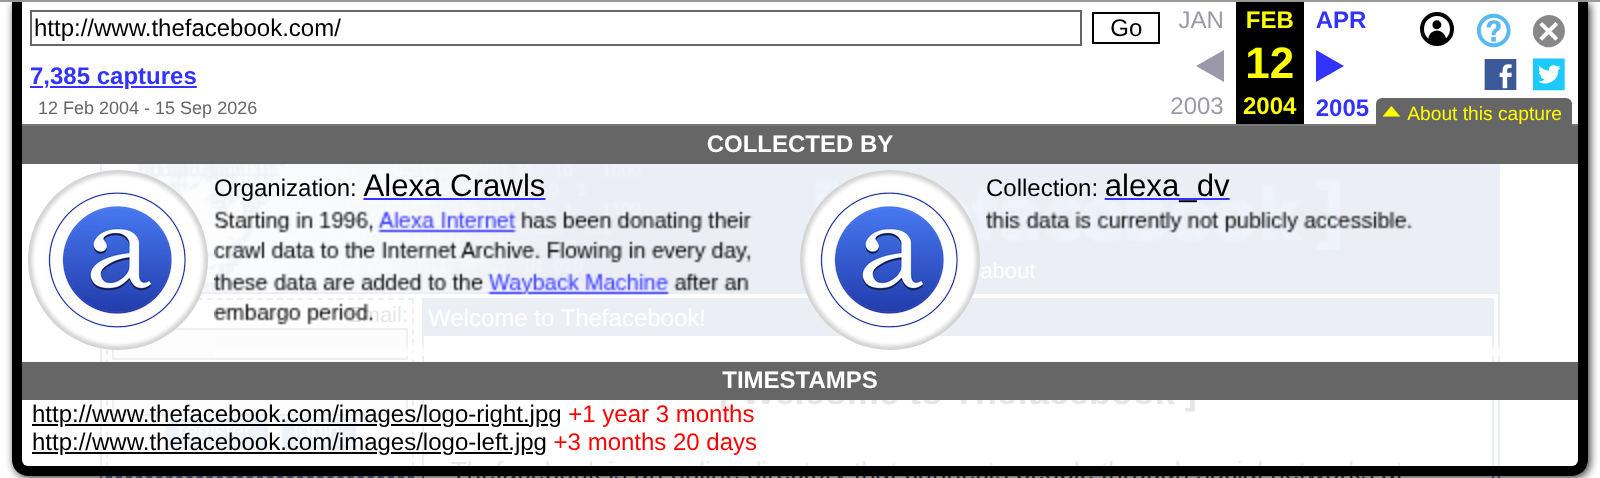
\includegraphics[width=.96\textwidth]{img/about_capture.png}
    \end{center}

    Click \textbf{About this capture} on the toolbar. \textbf{Collected by} names the organization and crawl that saved the page. \textbf{Timestamps} lists when each image, script, and stylesheet on it was saved.

    \bigskip
    The two logos on this February 12, 2004 capture of Thefacebook were saved \textbf{three months} and \textbf{more than a year} later.

    \bigskip
    An archived page is a composite: pieces from different moments, stitched together when you replay it.
\end{frame}

\begin{frame}{Reading the dots}
    \begin{columns}
        \begin{column}{0.6\textwidth}
            A dot's color is the HTTP status code the crawler got that day (Week~5):

            \medskip
            \textbf{Blue} --- 2xx, the page loaded\\
            \textbf{Green} --- 3xx, a redirect\\
            \textbf{Orange} --- 4xx, like 403 Forbidden or 404 Not Found\\
            \textbf{Red} --- 5xx, the server failed

            \bigskip
            facebook.com in 2005: blue until April 8, then a run of orange 403s, then blue again from August 6 --- now serving Thefacebook's homepage. The domain had changed hands.

            \bigskip
            Orange is not the archive failing. It faithfully recorded that the site said no.
        \end{column}
        \begin{column}{0.35\textwidth}
            \centering
            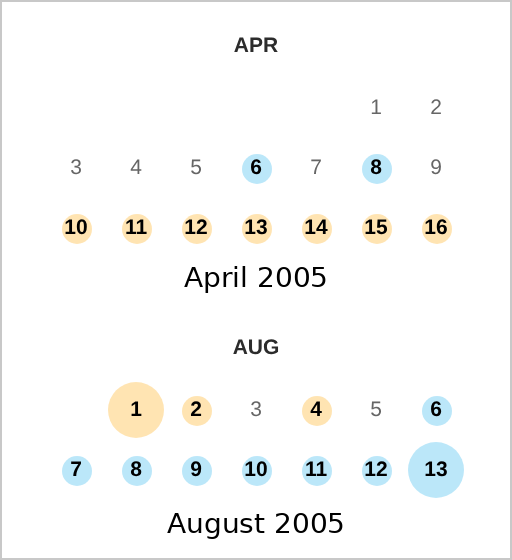
\includegraphics[width=\textwidth]{img/calendar_dots_2005.png}\\
            {\scriptsize facebook.com, 2005.}
        \end{column}
    \end{columns}
\end{frame}

\begin{frame}{Broken captures}
    \begin{columns}
        \begin{column}{0.6\textwidth}
            {\small \url{https://web.archive.org/web/19991114081850/http://x.com/}}

            \bigskip
            The HTML was saved on November 14, 1999. Its images were not.

            \bigskip
            Replay borrows each image from its nearest capture in time. Six of these seven have no good capture at all: the first ones, from August and September 2000, are all 404s.

            \bigskip
            Files served from another host --- \texttt{static.example.com}, a CDN --- have to be fetched on their own. Often they weren't.

            \bigskip
            URLs that JavaScript assembles while the page runs are often invisible to the crawler. Next week's problem.
        \end{column}
        \begin{column}{0.35\textwidth}
            \centering
            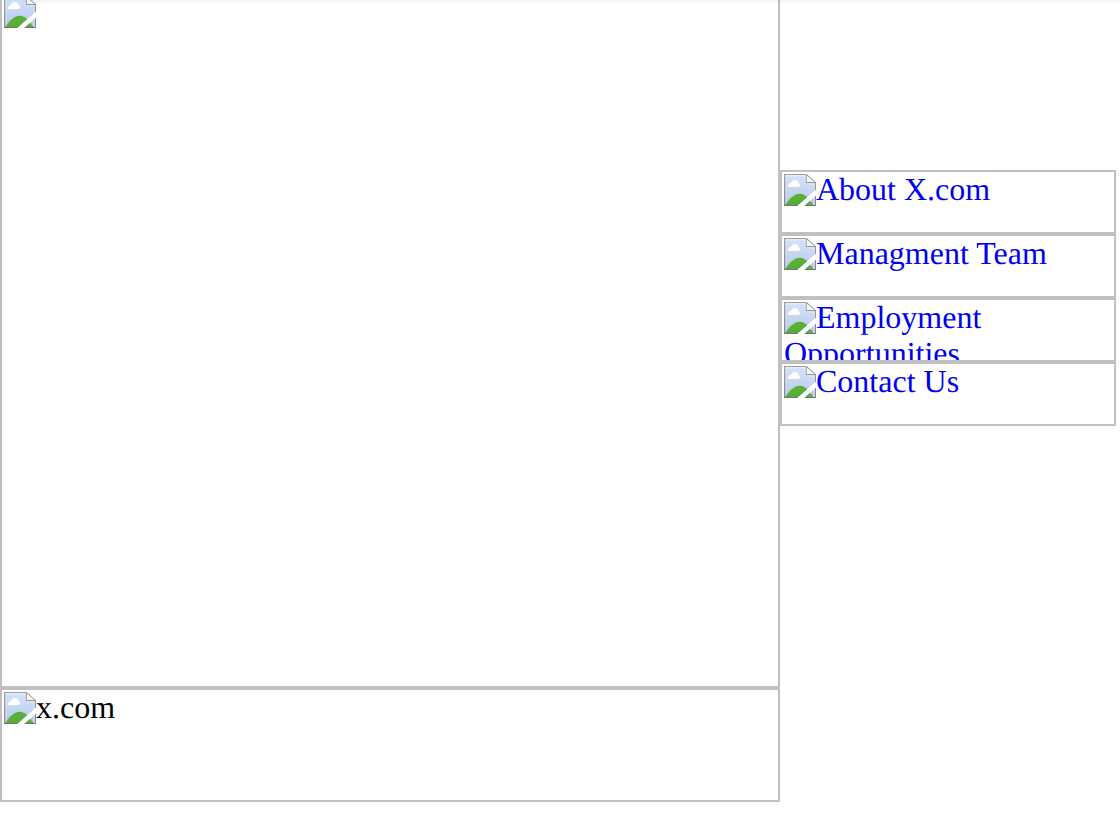
\includegraphics[width=\textwidth]{img/x_com_1999.png}\\
            {\scriptsize x.com, November 14, 1999.}
        \end{column}
    \end{columns}
\end{frame}

\begin{frame}{Missing captures}
    \begin{columns}
        \begin{column}{0.6\textwidth}
            Sometimes the Wayback Machine ``has not archived that URL.'' No crawler followed a link there, and nobody asked.

            \bigskip
            \textbf{Subdomains are separate sites.} \texttt{blog.example.com} can be missing while \texttt{example.com} has thousands of captures.

            \bigskip
            \textbf{Logins and paywalls} get saved as the login page.

            \bigskip
            \textbf{Exclusions.} Site owners can request to hide their pages.

            \bigskip
            \textbf{Soft 404s.} A blue dot can still be an error page, if the server sent it with a 200.
        \end{column}
        \begin{column}{0.35\textwidth}
            \centering
            
\includegraphics[width=\textwidth]{slides/week-07/img/archives-are-incomplete.jpg}\\
            {\footnotesize Obi-Wan logging onto the Wayback Machine}
        \end{column}
    \end{columns}
\end{frame}

\begin{frame}{Why some sites are archived better}
    \begin{center}
        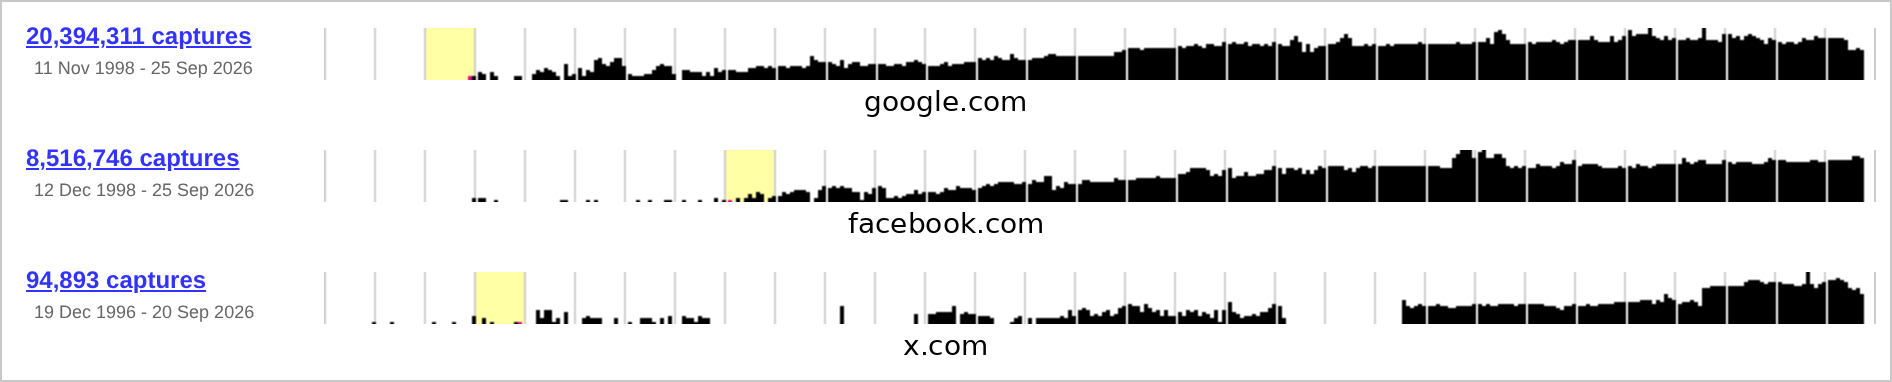
\includegraphics[width=.9\textwidth]{img/toolbar_counts.png}
    \end{center}

    google.com: more than 20 million captures. facebook.com: 8.5 million. x.com: 94,893. (September 2026)

    \bigskip
    Crawlers follow links, so well-linked, popular sites get found and revisited constantly. Captures also come from Save Page Now, volunteers rescuing dying sites (Archive Team), libraries (Archive-It), and special crawls like the End of Term archive of U.S.\ government sites at every presidential transition since 2008.

    \begin{alertblock}{Consequences}
        The archive is a sample, not a census. Popular, well-linked sites are over-represented --- and your sample inherits that.
    \end{alertblock}
\end{frame}

\begin{frame}{Why is it so slow?}
    \begin{columns}
        \begin{column}{0.6\textwidth}
            A nonprofit library serves more than a trillion archived pages, free, to anyone who asks.

            \bigskip
            It is also a target. In October 2024 a data breach and waves of DDoS attacks took the Wayback Machine offline for days.

            \bigskip
            And it is in court. It lost to book publishers in \textit{Hachette v.\ Internet Archive} (2024), and settled record labels' claim of up to \$621 million over its digitized 78s (2025).

            \bigskip
            Who should pay to remember the web?
        \end{column}
        \begin{column}{0.35\textwidth}
            \centering
            
\includegraphics[width=\textwidth]{img/wayback_down.png}\\
            {\scriptsize web.archive.org, while making this slide.}
        \end{column}
    \end{columns}
    \begin{alertblock}{Consequences}
        Be a polite client: pause between requests, retry with backoff when it fails, and cache what you download.
    \end{alertblock}
\end{frame}

\begin{frame}{The Inspector still works}
    \begin{columns}
        \begin{column}{0.5\textwidth}
            Right-click anything on an archived page and choose \textbf{Inspect}. Weeks 5 and 6 still apply: the DOM, selectors, attributes, tables.

            \bigskip
            The Archive adds a layer on top. \texttt{<div id="wm-ipp-base">} is its toolbar, and a comment marks \texttt{END WAYBACK TOOLBAR INSERT}. The original page starts right after.

            \bigskip
            Links stay inside the archive. Thefacebook's register link still carries a session ID from 2004: \texttt{register.php?PHPSESSID=df5154e5\ldots}
        \end{column}
        \begin{column}{0.45\textwidth}
            \centering
            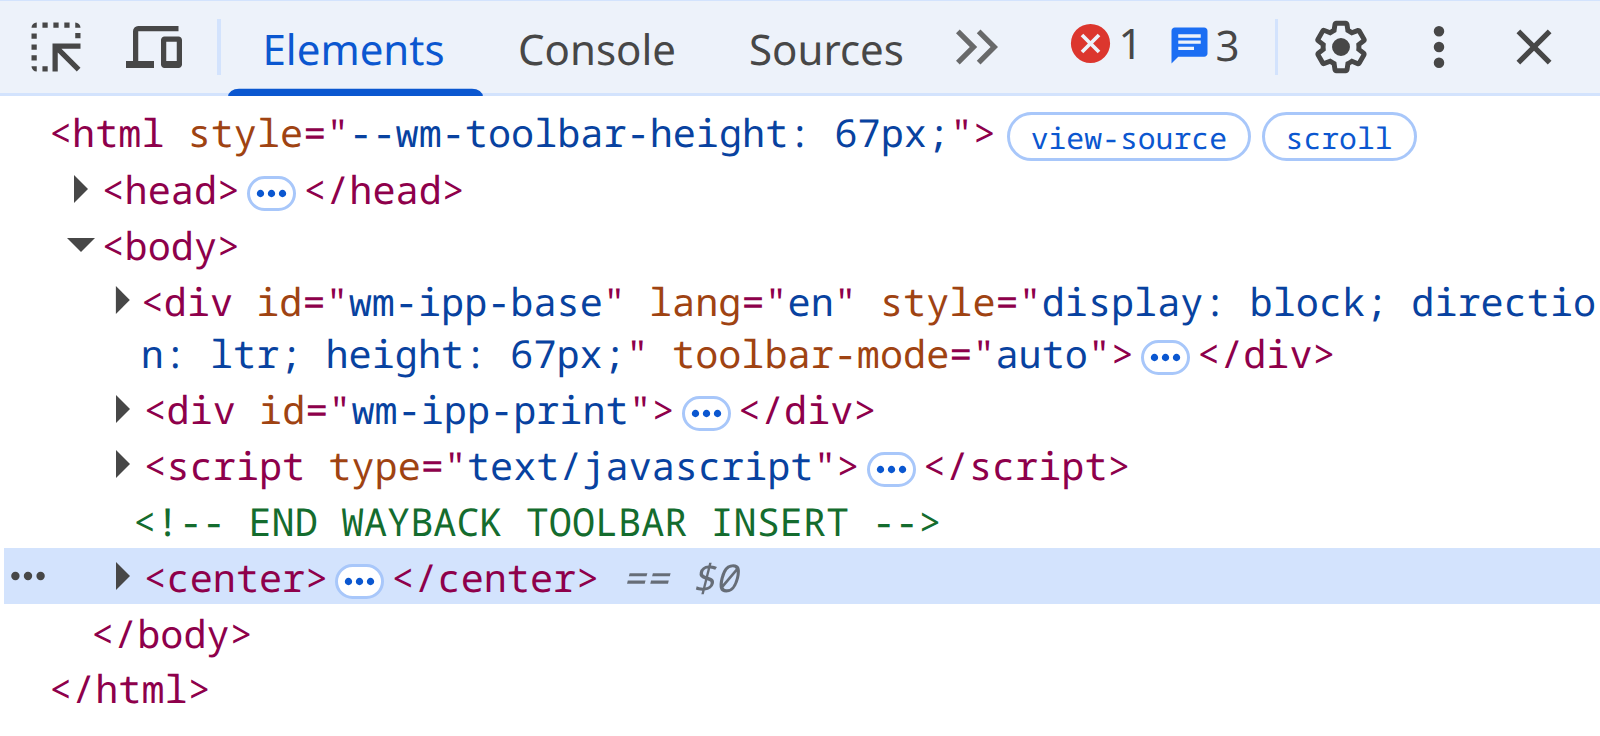
\includegraphics[width=\textwidth]{img/devtools_archived.png}\\
            {\scriptsize Chrome DevTools on Thefacebook, February 12, 2004.}
        \end{column}
    \end{columns}
\end{frame}

\begin{frame}{Raw or wrapped? The \texttt{id\_} rule}
    \begin{columns}
        \begin{column}{0.5\textwidth}
            What the Inspector shows is the \textit{wrapped} capture: the Archive's scripts in the \texttt{<head>}, its toolbar in the \texttt{<body>}, and links rewritten to stay in the archive.

            \bigskip
            Fine for browsing. Poison for measurement --- your counts of links, scripts, and images include the scaffolding.

            \bigskip
            Add \texttt{id\_} after the timestamp for the original bytes:\\
            {\scriptsize\texttt{.../web/20040212031928\textbf{id\_}/http://www.thefacebook.com/}}

            \bigskip
            Wednesday's measurement code fetches every page this way.
        \end{column}
        \begin{column}{0.48\textwidth}
            \centering
            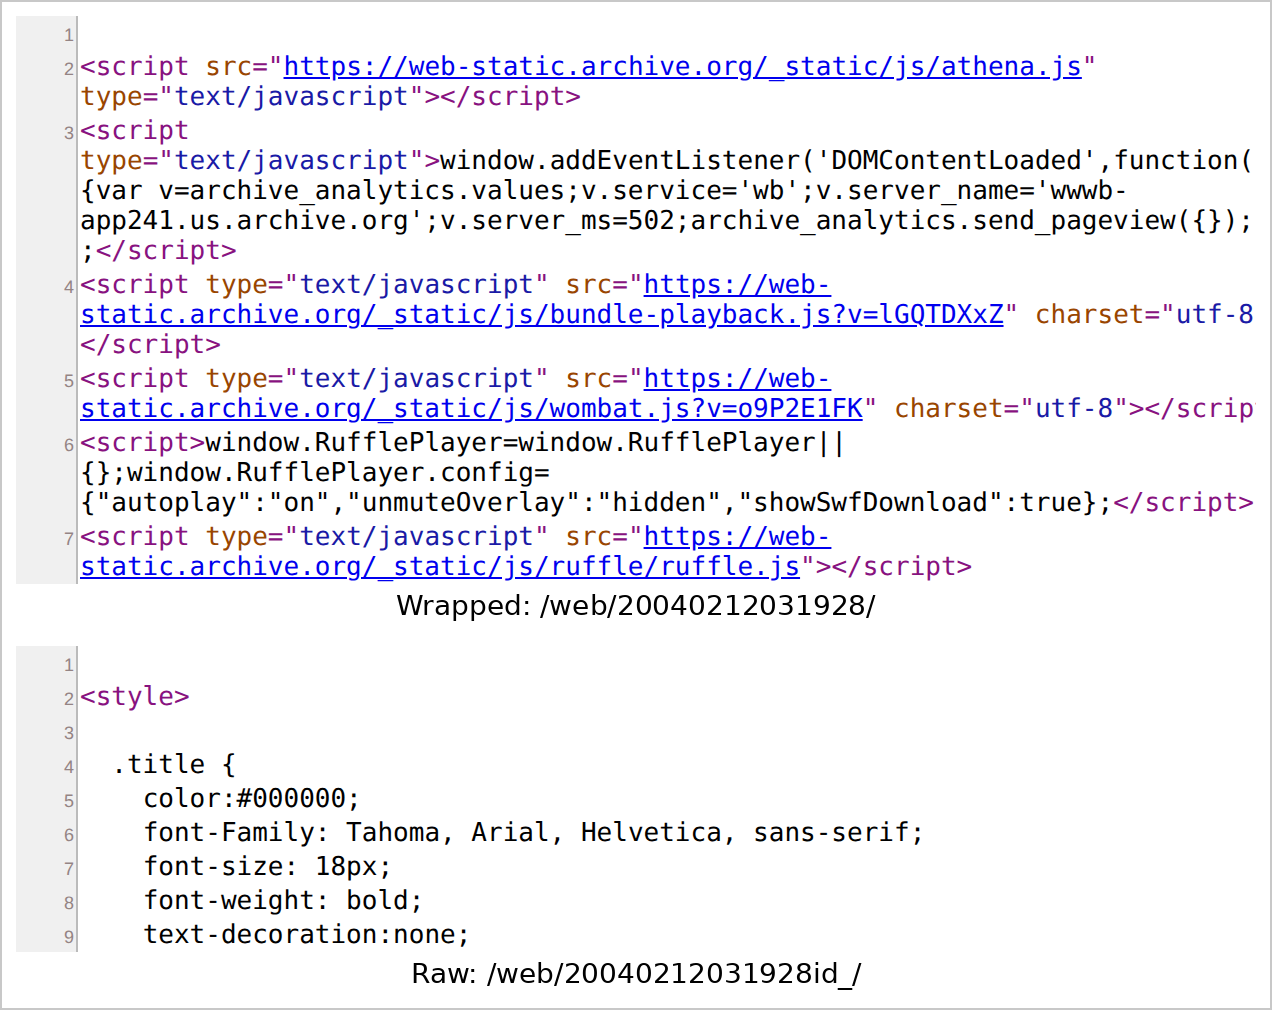
\includegraphics[width=\textwidth]{img/wrapped_vs_raw.png}\\
            {\scriptsize The same capture, wrapped (top) and raw (bottom).}
        \end{column}
    \end{columns}
\end{frame}

\begin{frame}{Facebook before Facebook}
    \begin{columns}
        \begin{column}{0.48\textwidth}
            \centering
            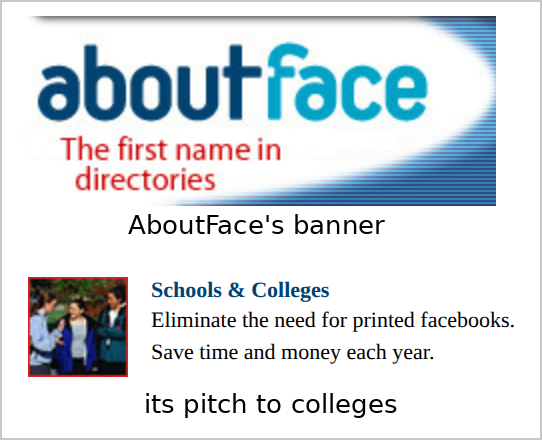
\includegraphics[width=.92\textwidth]{img/facebook_2004.png}\\
            {\scriptsize facebook.com, January 21, 2004.}
        \end{column}
        \begin{column}{0.48\textwidth}
            \centering
            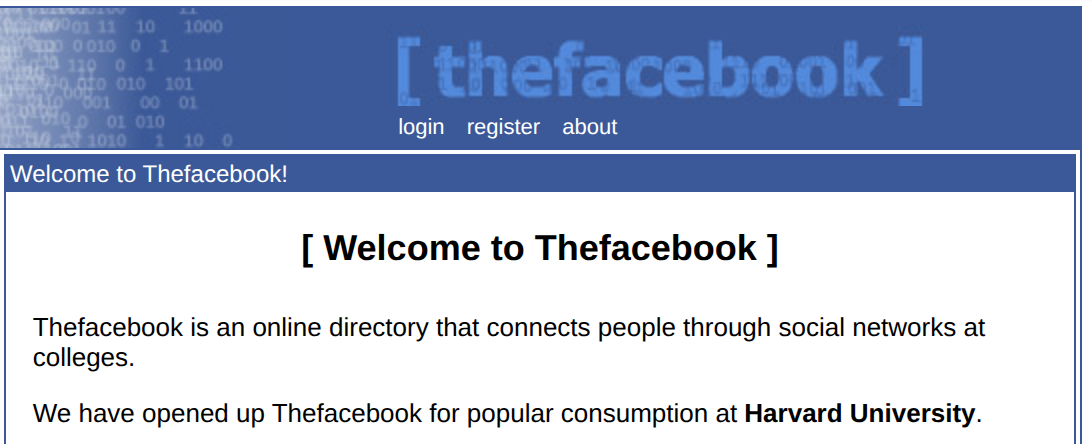
\includegraphics[width=.92\textwidth]{img/thefacebook_2004.png}\\
            {\scriptsize thefacebook.com, February 12, 2004.}
        \end{column}
    \end{columns}

    \bigskip
    Two weeks before Thefacebook launched, facebook.com belonged to AboutFace, ``The first name in directories.'' It sold software to help colleges ``eliminate the need for printed facebooks.''

    \bigskip
    Thefacebook bought the domain in 2005 for \$200,000 and dropped the ``The.''
\end{frame}

\begin{frame}{x.com before X}
    \begin{columns}
        \begin{column}{0.48\textwidth}
            \centering
            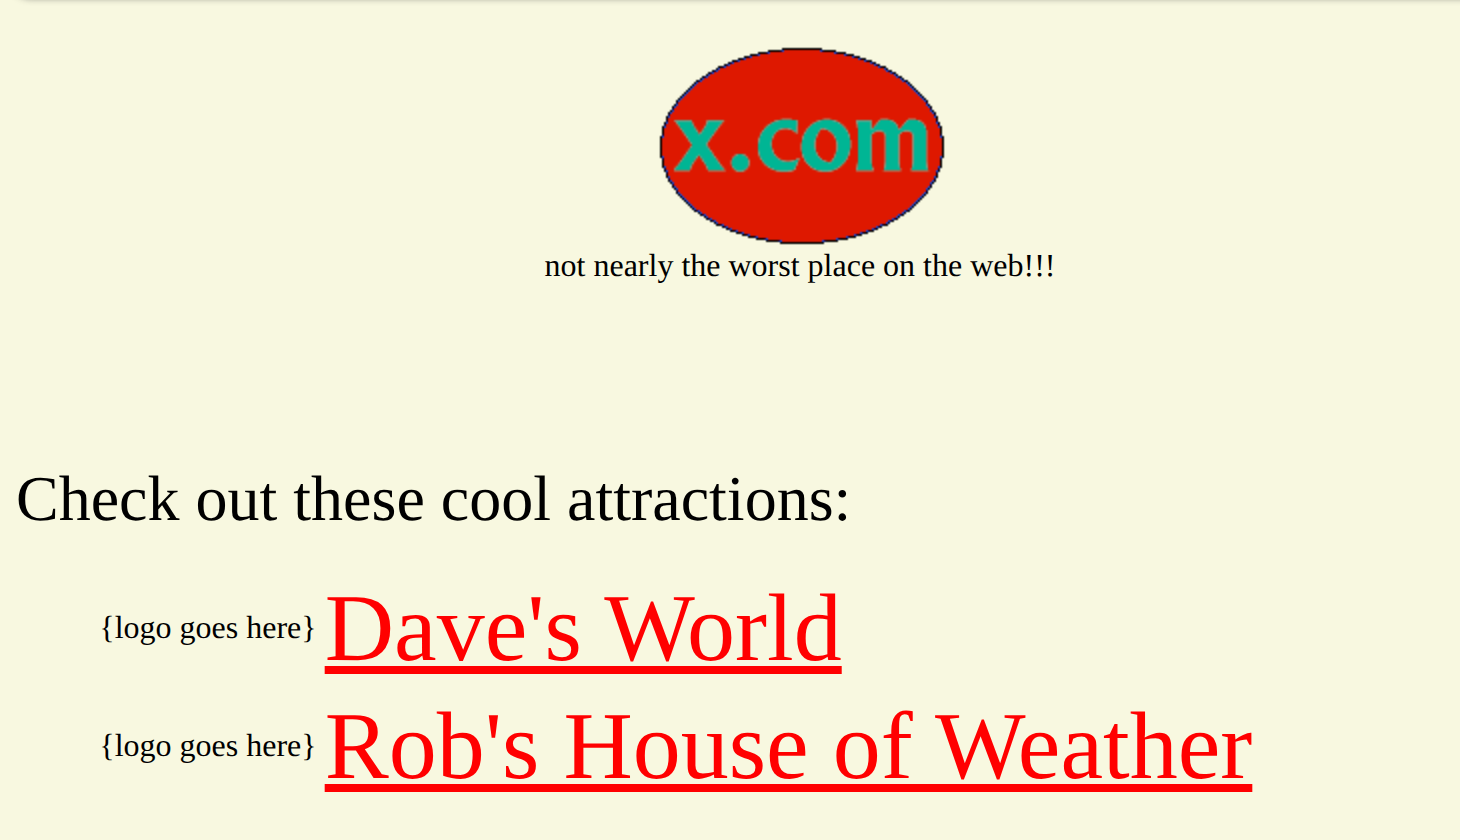
\includegraphics[width=\textwidth]{img/x_com_1997.png}\\
            {\scriptsize x.com, April 11, 1997.}
        \end{column}
        \begin{column}{0.48\textwidth}
            \centering
            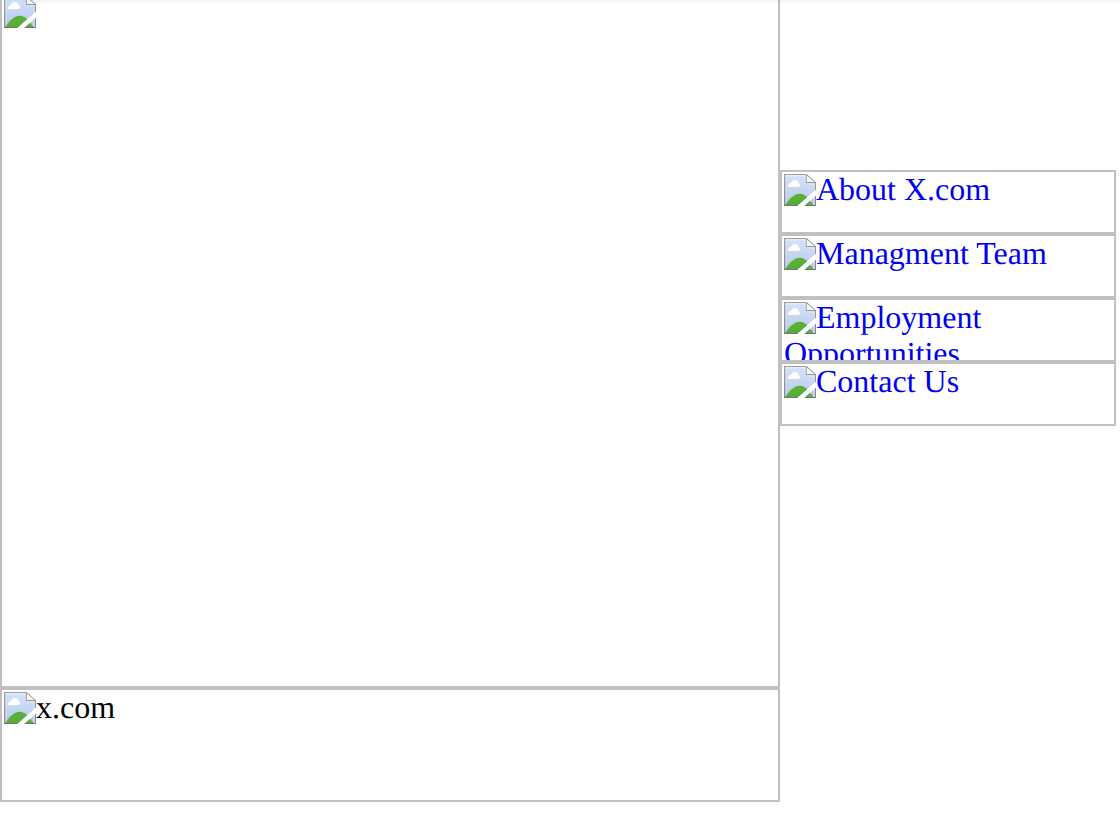
\includegraphics[width=.92\textwidth]{img/x_com_1999.png}\\
            {\scriptsize x.com, November 14, 1999.}
        \end{column}
    \end{columns}

    \bigskip
    1997: ``not nearly the worst place on the web!!!'' --- home of Dave's World and Rob's House of Weather.

    \bigskip
    1999: X.com, an online bank Elon Musk co-founded. It merged with Confinity, the company behind PayPal, in 2000. Musk bought the domain back from PayPal in 2017, and X, formerly Twitter, started using it in 2023.
\end{frame}

\begin{frame}{google.com, November 1998}
    \begin{center}
        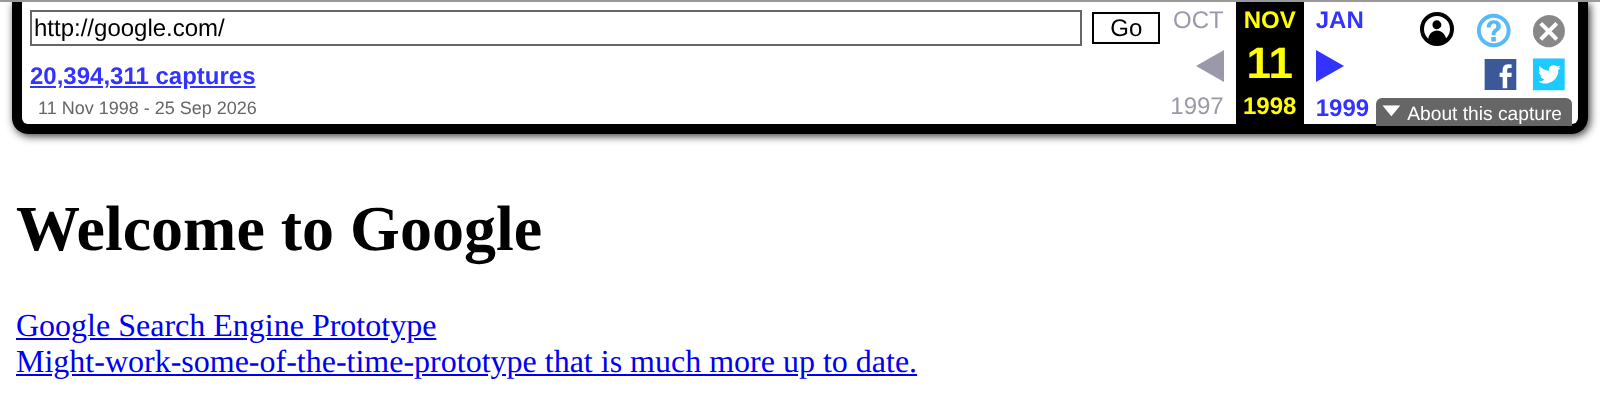
\includegraphics[width=.85\textwidth]{img/google_1998.png}
    \end{center}

    The oldest capture of google.com: a heading and two links.

    \bigskip
    ``Might-work-some-of-the-time-prototype that is much more up to date.''

    \bigskip
    More than twenty million captures later (September 2026).
\end{frame}

\begin{frame}{Research designs with the archived web}
    One old page is a curiosity. Many old pages, compared systematically, are data.

    \bigskip
    \begin{itemize}\small
        \item \textbf{One site, over time.} A platform's Terms of Service across twenty years --- Wednesday's notebook. Amos et al.\ (2021) did it for over a million privacy policies from more than 130,000 websites.
        \item \textbf{Many sites, over time.} How third-party tracking spread across the web from 1996 to 2016 (Lerner et al., 2016).
        \item \textbf{Disappearance itself.} Which pages rot, how fast, and where (Pew Research Center, 2024).
        \item \textbf{Before and after an event.} EDGI used the Wayback Machine to document climate-change language disappearing from federal websites in 2017.
    \end{itemize}

    \bigskip
    \textcite{arora_UsingWaybackMachine_2016} is a methods guide to mining websites this way.
\end{frame}

\begin{frame}{Internet Jones and the Echoes of the Lost Trackers}
    \begin{columns}
        \begin{column}{0.6\textwidth}
            Lerner, Kornfeld Simpson, Kohno, and Roesner (USENIX Security 2016) replayed archived pages from 1996 to 2016 and logged the third-party requests each one made.

            \bigskip
            Tracking grew in both prevalence and complexity, starting from the first tracker they found in 1996.

            \bigskip
            A big part of the paper measures where the archive's view of the past is imperfect --- today's failure modes --- and how to correct for it.
        \end{column}
        \begin{column}{0.35\textwidth}
            \centering
            
\includegraphics[width=.75\textwidth]{slides/week-07/img/train-bus.jpg}
        \end{column}
    \end{columns}
\end{frame}

\begin{frame}{Closing activity: time travel with the Wayback Machine}
    \begin{columns}
        \begin{column}{0.6\textwidth}\small
            \begin{enumerate}
                \item Pick a site that matters to you: your high school, your hometown paper, a game, a band. Find its earliest capture
                \item Find the capture closest to the day you were born
                \item Find a broken capture. Use About this capture or the Inspector to explain what broke
                \item Find the first capture where something changed: a logo, a slogan, a price. Open the capture halfway between two others. Repeat until you find the change
                \item Find a page the Archive does not have yet. Save it with Save Page Now
            \end{enumerate}

            \bigskip
            Stuck? Start with thefacebook.com, x.com, google.com, or colorado.edu

            \bigskip
            Report back with your oldest find, your weirdest find, and your most broken page
        \end{column}
        \begin{column}{0.35\textwidth}
            \centering
            
\includegraphics[width=\textwidth]{slides/week-07/img/elrond-i-was-there.jpg}\\
            {\footnotesize Loading the oldest snapshot on Wayback}
        \end{column}
    \end{columns}
\end{frame}

% =========================================================================
\section{Wednesday · Notebook Lab}
% =========================================================================

\begin{frame}[fragile]{Finding a snapshot --- the Availability API}
    The simplest question: does a snapshot exist near a date? Pass query args as a \texttt{params} dict so \texttt{requests} URL-encodes them (one value is itself a URL):
\begin{lstlisting}
import requests

api_url = "https://archive.org/wayback/available"
response = requests.get(api_url, params={"url": "https://www.cnn.com",
                                         "timestamp": "20000815"})  # Aug 15, 2000
data = response.json()

if data["archived_snapshots"]:
    snap = data["archived_snapshots"]["closest"]   # closest capture to that date
    print(snap["timestamp"], snap["url"])
else:
    print("No snapshot available near this date")
\end{lstlisting}
\end{frame}

\begin{frame}[fragile]{Retrieve it raw with \texttt{id\_}, then measure}
    Rewrite the snapshot URL to the \texttt{id\_} form, then parse it like any page:
\begin{lstlisting}
from bs4 import BeautifulSoup

ts = snap["timestamp"]
raw_url = snap["url"].replace(ts, ts + "id_")   # id_ -> original, unwrapped capture

soup = BeautifulSoup(requests.get(raw_url).text, "html.parser")
stats = {"year": ts[:4], "num_links": len(soup.find_all("a")),
         "num_scripts": len(soup.find_all("script"))}
\end{lstlisting}
    The same measurement across three eras tells the web's story:
\begin{lstlisting}
#   year  num_links  text_length  num_images  num_scripts
#   2000        150         8500          20            2   # largely static HTML
#   2024        800        45000         120           95   # a JS app that renders
\end{lstlisting}
\end{frame}

\begin{frame}[fragile]{The whole history --- the CDX Server API}
    Availability finds \textit{one} snapshot; CDX enumerates \textit{all} of them. Two params filter server-side --- less data, less cleanup:
    \begin{columns}
        \begin{column}{0.6\textwidth}
\begin{lstlisting}
cdx = "https://web.archive.org/cdx/search/cdx"
params = {"url": "facebook.com/terms",
          "output": "json",
          "fl": "timestamp,original,statuscode,length",
          "filter": "statuscode:200",  # only 200s
          "collapse": "digest"}        # drop repeats
data = requests.get(cdx, params=params).json()

df = pd.DataFrame(data[1:], columns=data[0])
df["timestamp"] = pd.to_datetime(
    df["timestamp"], format="%Y%m%d%H%M%S")
\end{lstlisting}
        \end{column}
        \begin{column}{0.35\textwidth}
            \centering
            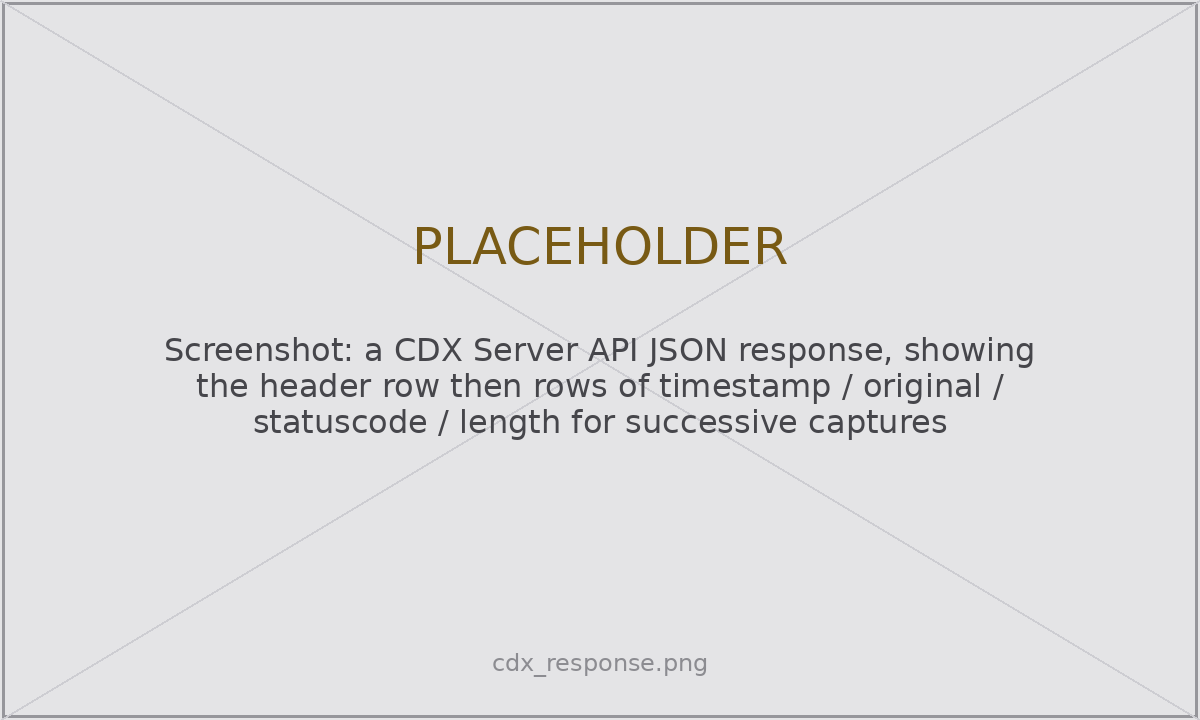
\includegraphics[width=\textwidth]{img/cdx_response.png}\\
            {\scriptsize Row 0 is the header; each later row is one distinct capture.}
        \end{column}
    \end{columns}
\end{frame}

\begin{frame}[fragile]{Tracking a document over time}
    Wrap the Availability + \texttt{id\_} + parse steps in \texttt{get\_wayback\_content()} (returns \texttt{None} on a miss), then loop over quarterly dates:
\begin{lstlisting}
dates = pd.date_range(start="2005-01-01", end="2024-01-01", freq="QS")

results = []
for date in dates:
    snap = get_wayback_content("facebook.com/terms", date)
    if snap is not None:          # skip misses instead of crashing the run
        results.append(snap)
    time.sleep(1)                 # rest between requests -- the Archive is a nonprofit
# Retrieved 68 snapshots from 77 time points
\end{lstlisting}
    Serialize immediately --- you may not be able to re-scrape it later:
\begin{lstlisting}
import json
with open("fb_tos_history.json", "w") as f:
    json.dump(results, f, indent=2)   # (also cache each raw capture as you go)
\end{lstlisting}
\end{frame}

\begin{frame}[fragile]{Measuring change --- bag-of-words}
    Represent each version as a vector of word frequencies (order ignored), then compare vectors. Install once with \texttt{conda install -c conda-forge gensim nltk}; pip has no ready-made gensim for Python 3.14 yet.
\begin{lstlisting}
from gensim.utils import simple_preprocess
from gensim import corpora, similarities
from nltk.corpus import stopwords          # nltk.download("stopwords") once

stop = set(stopwords.words("english"))
docs = [[t for t in simple_preprocess(r["content"]) if t not in stop] for r in results]

dct = corpora.Dictionary(docs)             # word -> id
corpus = [dct.doc2bow(d) for d in docs]    # each version -> word-count vector
index = similarities.SparseMatrixSimilarity(corpus, num_features=len(dct))
change = [1 - index[corpus[i-1]][i] for i in range(1, len(corpus))]  # 0=same, 1=all-new
\end{lstlisting}
    Plotting \texttt{change} over time gives a change timeline: spikes flag major revisions --- a new policy, a redesign, a response to controversy.
\end{frame}

\begin{frame}{Lab: work these, then show-and-tell}
    \begin{columns}
        \begin{column}{0.6\textwidth}
            Work in pairs. Do these exercises from the notebook:
            \begin{enumerate}\small
                \item Select a policy document. Get 5 or more versions from different dates. Plot the length of each version.
                \item Use the CDX API. Compare the capture frequency and the page size of two competing organizations.
                \item Calculate the similarity between all pairs of versions. Make a heatmap. Identify the points of change.
                \item Examine the archive history of a government site. Report the gaps, the coverage, and the change in size.
                \item Compare the earliest snapshot with the most recent snapshot. Write 200 words about the differences.
                \item[6.] \textbf{5617}: assess the limits of the Wayback Machine. Include the toolbar, the capture bias, and the gaps. Compare your results with \textcite{rogers2019doing}
            \end{enumerate}
        \end{column}
        \begin{column}{0.35\textwidth}
            \begin{block}{Show-and-Tell}
                \footnotesize Bring one of these to class:
                \begin{itemize}\footnotesize
                    \item a bug that you could not solve
                    \item a change you found in the archived past
                    \item a question for a research design
                \end{itemize}
            \end{block}
        \end{column}
    \end{columns}
\end{frame}

% =========================================================================
\section{Friday · Textbook Revisions}
% =========================================================================

\begin{frame}{Improving Chapter 7 together}
    \begin{columns}
        \begin{column}{0.6\textwidth}
            Today we make the book better. Each of you opens a \textbf{pull request} against \texttt{ch-07-archives.qmd} and reviews a classmate's.

            \bigskip

            The workflow (from Week 1):
            \begin{enumerate}\small
                \item Branch / fork the book repo
                \item Edit the chapter; commit with a clear message
                \item Open a PR describing \textit{what} and \textit{why}
                \item Review two peers' PRs: kind, specific, actionable
            \end{enumerate}
        \end{column}
        \begin{column}{0.35\textwidth}
            \centering
            
\includegraphics[width=\textwidth]{img/pr_review.png}
        \end{column}
    \end{columns}
\end{frame}

\begin{frame}{A revision menu for Chapter 7}
    High-value targets --- pick one and scope it to a single PR:
    \begin{itemize}
        \item \textbf{Run it against the live APIs.} The comparison numbers and ``68 of 77 snapshots'' are \textit{illustrative}. Query the real Availability/CDX endpoints, report actual results, and label sample outputs as representative.
        \item \textbf{Add a figure for the APIs.} The new figures cover the Wayback interface, but the Availability and CDX sections are still all code. An annotated CDX response would anchor them.
        \item \textbf{Close a gap in ``Common Issues to Debug.''} A worked \texttt{id\_} example (link counts wrapped vs.\ raw), a copy-paste \texttt{nltk.download("stopwords")} recipe, or a CDX missing-field case.
        \item \textbf{Make an exercise self-checking.} Add expected output, a rubric, or a starter cell to the open-ended policy-tracking and heatmap exercises.
        \item \textbf{Add a research design.} The chapter's research-designs section lists four. Add a fifth from your own field, with a citation --- \textcite{brugger_SAGEHandbookWeb_2018} is a good place to look.
    \end{itemize}
\end{frame}

\begin{frame}{A good revision, and a good review}
    \begin{columns}
        \begin{column}{0.6\textwidth}
            \begin{block}{A strong PR}
                \begin{itemize}\small
                    \item One focused change, clearly titled
                    \item Explains the problem it fixes
                    \item Builds (\texttt{quarto render}) without errors
                    \item Matches the book's voice and notation
                    \item Discloses any AI assistance
                \end{itemize}
            \end{block}
        \end{column}
        \begin{column}{0.35\textwidth}
            \begin{block}{A strong review}
                \begin{itemize}\small
                    \item Runs / reads the change, not just skims
                    \item Names specifics (line, claim, code)
                    \item Separates ``must fix'' from ``nice to have''
                    \item Is generous --- assume good faith
                    \item Ends with a clear verdict
                \end{itemize}
            \end{block}
        \end{column}
    \end{columns}
    \medskip
    \centering\small Next week: \textbf{Dynamic pages} --- when the data appears only after JavaScript runs (Selenium).
\end{frame}

% =========================================================================
\begin{frame}{Key takeaways}
    \begin{enumerate}
        \item The web is impermanent (link rot); the \textbf{Internet Archive} is public infrastructure that preserves it.
        \item \textbf{Availability API} finds one snapshot near a date; the \textbf{CDX Server} enumerates the full history --- filter and collapse server-side.
        \item Append \texttt{id\_} for the \textbf{raw} capture; the toolbar-wrapped version pollutes every measurement.
        \item Wayback $+$ text analysis turns the archive into \textbf{longitudinal data} --- measure change, don't just observe it.
        \item Be a good citizen: \texttt{sleep} between requests, cache raw captures, and \textbf{serialize} --- you may not be able to re-scrape.
    \end{enumerate}
    \bigskip
\end{frame}

\end{document}
